\chapter{One-shot Detail Retouching}\label{one-shot}

 Photo retouching is a difficult task for novice users as it requires expert knowledge and advanced tools. Photographers often spend a great deal of time generating high-quality retouched photos with intricate details. In this paper, we introduce a one-shot learning based technique to automatically retouch details of an input image based on just a single pair of before and after example images. Our approach provides accurate and generalizable detail edit transfer to new images. We achieve these by proposing a new representation for image to image maps. Specifically, we propose neural field based transformation blending in the patch space for defining patch to patch transformations for each frequency band. This parametrization of the map with anchor transformations and associated weights, and spatio-spectral localized patches, allows us to capture details well while staying generalizable. We evaluate our technique both on known ground truth filters and artist retouching edits. Our method accurately transfers complex detail retouching edits.



\begin{figure}
  \includegraphics[width=\textwidth]{Chapters/detail-retouching-figs/teaser_CVMP.pdf}
  \caption{Our technique automatically transfers retouching edits to new images by learning the desired edits from one example \textit{before-after} pair (insets). The transferred edits accurately capture intricate details such as wrinkles, dark spots, strands of hair, or eyelashes, as shown in the input (top) and retouched (bottom) pairs. Image courtesy of Jenavieve (top-left), Logan ProPro (top-left, inset), Marissa Oosterlee (top-middle). (CC-BY).}
  % \Description{Our technique automatically transfers retouching edits to new images by learning the desired edits from one example \textit{before-after} pair (insets). The transferred edits accurately capture intricate details such as wrinkles, dark spots, strands of hair, or eyelashes, as shown in the input (top) and retouched (bottom) pairs.}
  \label{fig:teaser}
\end{figure}


% \received{20 February 2007}
% \received[revised]{12 March 2009}
% \received[accepted]{5 June 2009}






\section{Introduction}\label{sec:introduction}

Photo retouching is often desirable as it improves the aesthetic quality of photographs by eliminating imperfections and \nobreak highlighting subjects of interest. Even with significant progress in digital photography owing to advancements in camera sensors and image processing algorithms, professional retouches via manual adjustments are still needed to achieve a desired look. These artistic edits require considerable manual effort as they consist of global adjustments, such as brightening and contrast enhancement, as well as fine edits applied to local regions. Professionals spend a great deal of time to generate such edits, which motivates us to automatically mimic a specific style or type of retouch.

The development of automatic photo retouching tools can be helpful for both novice users and experts as it offers a basis for a professional retouching style. However, automating detailed edits of professionals is challenging as their editing pipelines are spatially varying, context-aware, and highly nonlinear, containing per-pixel adjustments. Recent learning-based methods address this complexity in image-to-image translation by proposing local context-aware methods, such as pixel-adaptive neural network architectures \cite{shaham2021spatially, li2020lapar}, learning parameters of local filters \cite{moran2020deeplpf}, or multi-stream models to extract global and local features separately \cite{Gharbi17Deep}. However, these data-driven methods require a large dataset of matching example image pairs. Even then, the mappings are sensitive to segmentation errors, unseen semantic regions, and image content~\cite{yan2016automatic}. %Many successful methods require example and input images to be content-wise pixel-level aligned to achieve plausible results \cite{Shih14Style}.

% in intricate details 
The gap between manual and automatic enhancement motivates me to develop a novel photo retouching technique that can learn global and local adjustments from just \emph{a single example image pair}. The proposed method thus sidesteps the need for large datasets, which are very difficult to obtain for the detail retouching task. Users are allowed to choose one example \emph{before-after} pair from which the model learns the underlying retouching style. Subsequently, the retouching edit can be applied to a different input image.

Here, we assume that example and input images share similar local content. The user can thus decide on the semantics of the example and input photos and the structural changes to be transferred. This is easy for humans and practical for many scenarios, e.g. face edits transferred to faces. The framework then handles the difficult part for humans: capturing how fine details change in an edit and applying those automatically to a new image. The method can further be combined with brushes if fully automatic transfers are not desired. 

This is achieved by defining the retouching problem as a map given by a \emph{spatio-spectral patch-space neural field based transformation blending}. This representation is primarily inspired by professional detail retouching pipelines as I elaborate on in Section \ref{chap:motivations}. This map representation is composed of learned patch maps at multiple scales, i.e. frequency bands. Each of these maps is represented by a number of \emph{transformation matrices} blended with \emph{patch-adaptive weights} that are learned by a multilayer perceptron. I jointly optimize the transformation matrices and corresponding weights for each band. This representation captures edits to details better than any previous techniques while staying generalizable to new images. It is also simple enough to be extended in many different ways in future works.

In summary, there are two main contributions of this work: 

%Multiple Transformation Blending
\begin{itemize}

    \item \textbf{A novel patch-space image map representation} as a weighted blending of transformation matrices with neural fields.
    
	\item \textbf{A one-shot detail retouching algorithm} that allows transfer of edits to details to new images based on a single before-after image pair.

\end{itemize}


\section{Related work}

Photo retouching has been explored in image processing and computer vision communities under different domains, such as photo enhancement and image-to-image translation. Below, we first discuss recent methods on photo enhancement and then image-to-image map definitions with the main focus on learning-based methods.

\subsection{Digital photo enhancement}
% \myworries{Check Rafals' paper -- is it global tone mapping, where to put it in the related work}
\paragraph{Global image enhancement.} Colour and tone transfer has been considered a very effective technique to improve the perceptual quality of photos with pre-defined rules or examples \cite{Faridul14ASurvey, mustafa2022distilling}. 

Earlier methods typically apply global changes and adjust image statistics \cite{Bychkovsky11Learning, Bae06Two, Pitie05NDimensional,Pitie07Automated,Reinhard01Color,Sunkavalli10Multi, he2020conditional, park2018distort}, e.g., mean and standard deviation, without considering image content and local variations \cite{CohenOr06Color}. These methods, in general, transfer colour changes, ignoring edits in fine details. On the other hand, the proposed method learns a mapping per frequency band, capturing transfers even in high frequencies. \citeauthor{Bychkovsky11Learning} \cite{Bychkovsky11Learning} collected the MIT-Adobe FiveK dataset of 5,000 photographs and their retouched versions by five artists. The authors propose a regression model to learn artists' retouching styles from before-retouched pairs. \citeauthor{chen2017fast} \cite{chen2017fast} introduce a fully-convolutional neural network model to learn global image processing operators, such as photographic style, nonlocal dehazing, and pencil drawing. \citeauthor{Hu18Exposure} \cite{Hu18Exposure} presents a photo retouching pipeline for various post-processing operations, where global adjustment curves are approximated. The authors propose a deep reinforcement learning approach to model users' edit preferences from a given photo collection. 
 
Nevertheless, global transfers cannot capture local and regional variations in a photo \cite{CohenOr06Color}.They may result in artifacts when the local target regions of the example and input images do not match. In this method, we adapt the mappings to each image patch separately, thus accurately capturing local edits in intricate details.

\paragraph{Local context-aware image enhancement.} 
 To capture local variations, different methods have been proposed, such as learning local representative color transform \cite{kim2021representative}, estimating an image-to-illumination mapping with a local feature extractor \cite{wang2019underexposed}, local histogram matching \cite{Shapira13Image}, segmentation \cite{Laffont14Transient,Tai07Soft}, combining and learning pre-defined filters \cite{Berthouzoz11AFramework,Chen18Deep,Huang14Parametric,Omiya18Learning,Saeedi18Multimodal} or with further user guidance \cite{An10User,Pouli11Progressive,Tai05Local}, detection or learning of image semantics and context \cite{Gharbi17Deep,Hwang12Context,Kaufman12Content,Nam17Deep,Yan14Automatic,Zhu18Automatic}, matching \cite{HaCohen11Nonrigid}, or precise alignment \cite{Kagarlitsky09Piecewise, Shih13Data}. 
 
 Furthermore, recent work has focused on learning global and local adjustments via spatially-varying filters \cite{moran2020deeplpf, Gharbi17Deep, chen2018deep, shaham2021spatially, li2020lapar}. \citeauthor{chen2018deep} \cite{chen2018deep} introduce a global feature extraction layer along with per-pixel adjustments to enhance photos. Bilateral guided joint upsampling \cite{chen2016bilateral} also allows for local and global image processing with an encoder-decoder approach. HDRNet \cite{Gharbi17Deep} learn content-aware, global, and local adjustments via a two-stream convolutional architecture, which extracts local and global features separately to fit local affine transformations and encode the high-level description of images, respectively. Also, \citeauthor{moran2020deeplpf} \cite{moran2020deeplpf} propose to learn the parameters of three different spatially local filters to automatically enhance photos. 

Local color and tone adjustments might still be insufficient to capture intricate details \cite{Bae06Two}. Transfer of such details typically requires a dense matching \cite{HaCohen11Nonrigid} or alignment between example and input images \cite{Shih14Style}. To achieve either dense matching or alignment, methods constrain their datasets to contain very similar example and input images, for example, faces with similar characteristics and views~\cite{Shih14Style}. On the other hand, this framework does not require dense correspondences between input and example images but still transfers intricate details. It accurately represents such complex mappings with an operator summing the effects of various transformations multiplied with corresponding patch-adaptive weights, applied at multiple frequency bands.

\paragraph{Differentiable image processing pipelines.}
To have more flexibility and control over the rendering process, methods based on image signal processors (ISP)s have been proposed to enhance photos. In both \cite{tseng2019hyperparameter, yu2021reconfigisp}, hyperparameters of an ISP are optimized. Different from \cite{tseng2019hyperparameter}, which only applies to a fixed pipeline, \citeauthor{yu2021reconfigisp} \cite{yu2021reconfigisp} can explore different ISP architectures. Furthermore, \citeauthor{tseng2022neural} \cite{tseng2022neural} model a commercial raw processing pipeline with a series of neural networks to render sRGB images from raw inputs. As we assume example and input images to be processed RGB images rather than raw data, I refrain from comparing our method with such ISP-based methods.


\subsection{Defining maps between images}

\paragraph{Unsupervised methods.} Some learning-based techniques only require one or more examples of retouched photos without their before examples to learn the transfer. Such unsupervised methods capture a certain style by decomposing images into a reflection map and an illumination map~\cite{ma2021retinexgan},
extracting and recomposing band representations of training images~\cite{yang2020fidelity}, regularizing unpaired training using information extracted from the input~\cite{9334429}, segmenting the image into semantic regions~\cite{Liu16Makeup}, adaptive image regions~\cite{Frigo16Split}, learning semantic and global features~\cite{Chen18Deep}, progressively translating image from coarse to fine via pyramids of generative models \cite{lin2020tuigan}, or utilizing artistic principles and pre-defined filters~\cite{Zhang13Style,Hu18Exposure}. These methods transfer pre-defined elements of the desired style, or global color and tone. Defining the desired style and the content of the input image that is to remain is challenging. Hence, these methods typically assume prior knowledge of the type of desired adjustments. Even then, capturing the retouching edits in details remains out of scope since these methods are mainly designed for domain transfer, working on high level features of images. % TuiGAN: compare with our work, discuss how bady they perform in details although they work as single-shot --

As a weakly supervised method, \citeauthor{visual_attribute} \cite{visual_attribute} propose a technique based on image analogy \cite{Hertzmann01Image} to transfer the visual attributes, such as color, tone, texture, and style, across images that look very different but share similar semantic structures. Similar to this work, they also work with one example pair (A and B') to transfer the attributes. However, they rather focus on high-level features, disregarding the edits in intricate details.

\paragraph{Supervised methods.} 
For a conceivable representation, many supervised transfer methods require a large dataset of well-aligned example image pairs whose contents are very similar \cite{kim2021representative, wang2019underexposed}. However, finding or generating such a dataset is difficult as the content of images can change dramatically. Even with such a dataset, segmentation errors, unseen semantic regions, or image content can still change the results significantly \cite{10.1145/2790296}. In contrast, this framework allows users to choose the example pairs from which the desired style is learned, hence sidestepping the challenging semantics problem. Similar content and structures between example and input images lead to more natural transfers.


Convolutional neural networks (CNNs) are the de-facto model for image processing with supervised learning methods. While CNNs present state-of-the-art results in computer vision tasks, they are not required \cite{tolstikhin2021mlp}. MLP-based architectures have recently gained popularity in image classification and image-to-image translation. \citeauthor{cazenavette2021mixergan} \cite{cazenavette2021mixergan} propose the MLP-Mixer architecture that only uses simple MLP blocks to learn image classification. \citeauthor{cazenavette2021mixergan} \cite{cazenavette2021mixergan} also show an application of an MLP-based architecture for image synthesis. They adapt the MLP-Mixer architecture \cite{tolstikhin2021mlp} to perform unpaired image-to-image translation. The fact that MLP-based architectures attain competitive results in challenging vision tasks motivated me to explore the use of an MLP block as an alternative to CNNs in the context of photo retouching.

\section{Overview and motivations}
\label{chap:motivations}

Given a pair of example images $X$ and $Y$, the aim is to learn a map $M$ such that $Y = M(X)$. The learned map can then be applied to a new input image $I$ to obtain the retouched output $O = M(I)$. 

The map is defined by 1) decomposing the example images into multiple feature maps $X_l$, $Y_l$ capturing details at different scales, such as coefficients at different bands of a Laplacian pyramid. 2) learning a separate mapping $M_l$ for each $X_l$, $Y_l$ pair in the patch space as a blending of transformation matrices with neural field based weights, all learned jointly. The overall map representation is illustrated in Figure~\ref{fig:modelT}.

For the transfer of edits, the $M_l$ are computed and applied to each patch of the decomposition $I_l$ of an input image $I$ to obtain the corresponding output patch of $O_l$. The patches are finally placed at their spatial locations and averaged to reconstruct each band $O_l$, which are summed to get the output image $O$.

The motivation behind designing such a map representation with frequency decomposition and transformation blending comes from studying the nature of retouching edits. 
\begin{itemize}
\item First, artists often decompose images into different frequency bands to have better control over structural and textural edits to details. For instance, they filter out the low frequency components to better enhance the details:

\begin{figure}[ht]
\centering
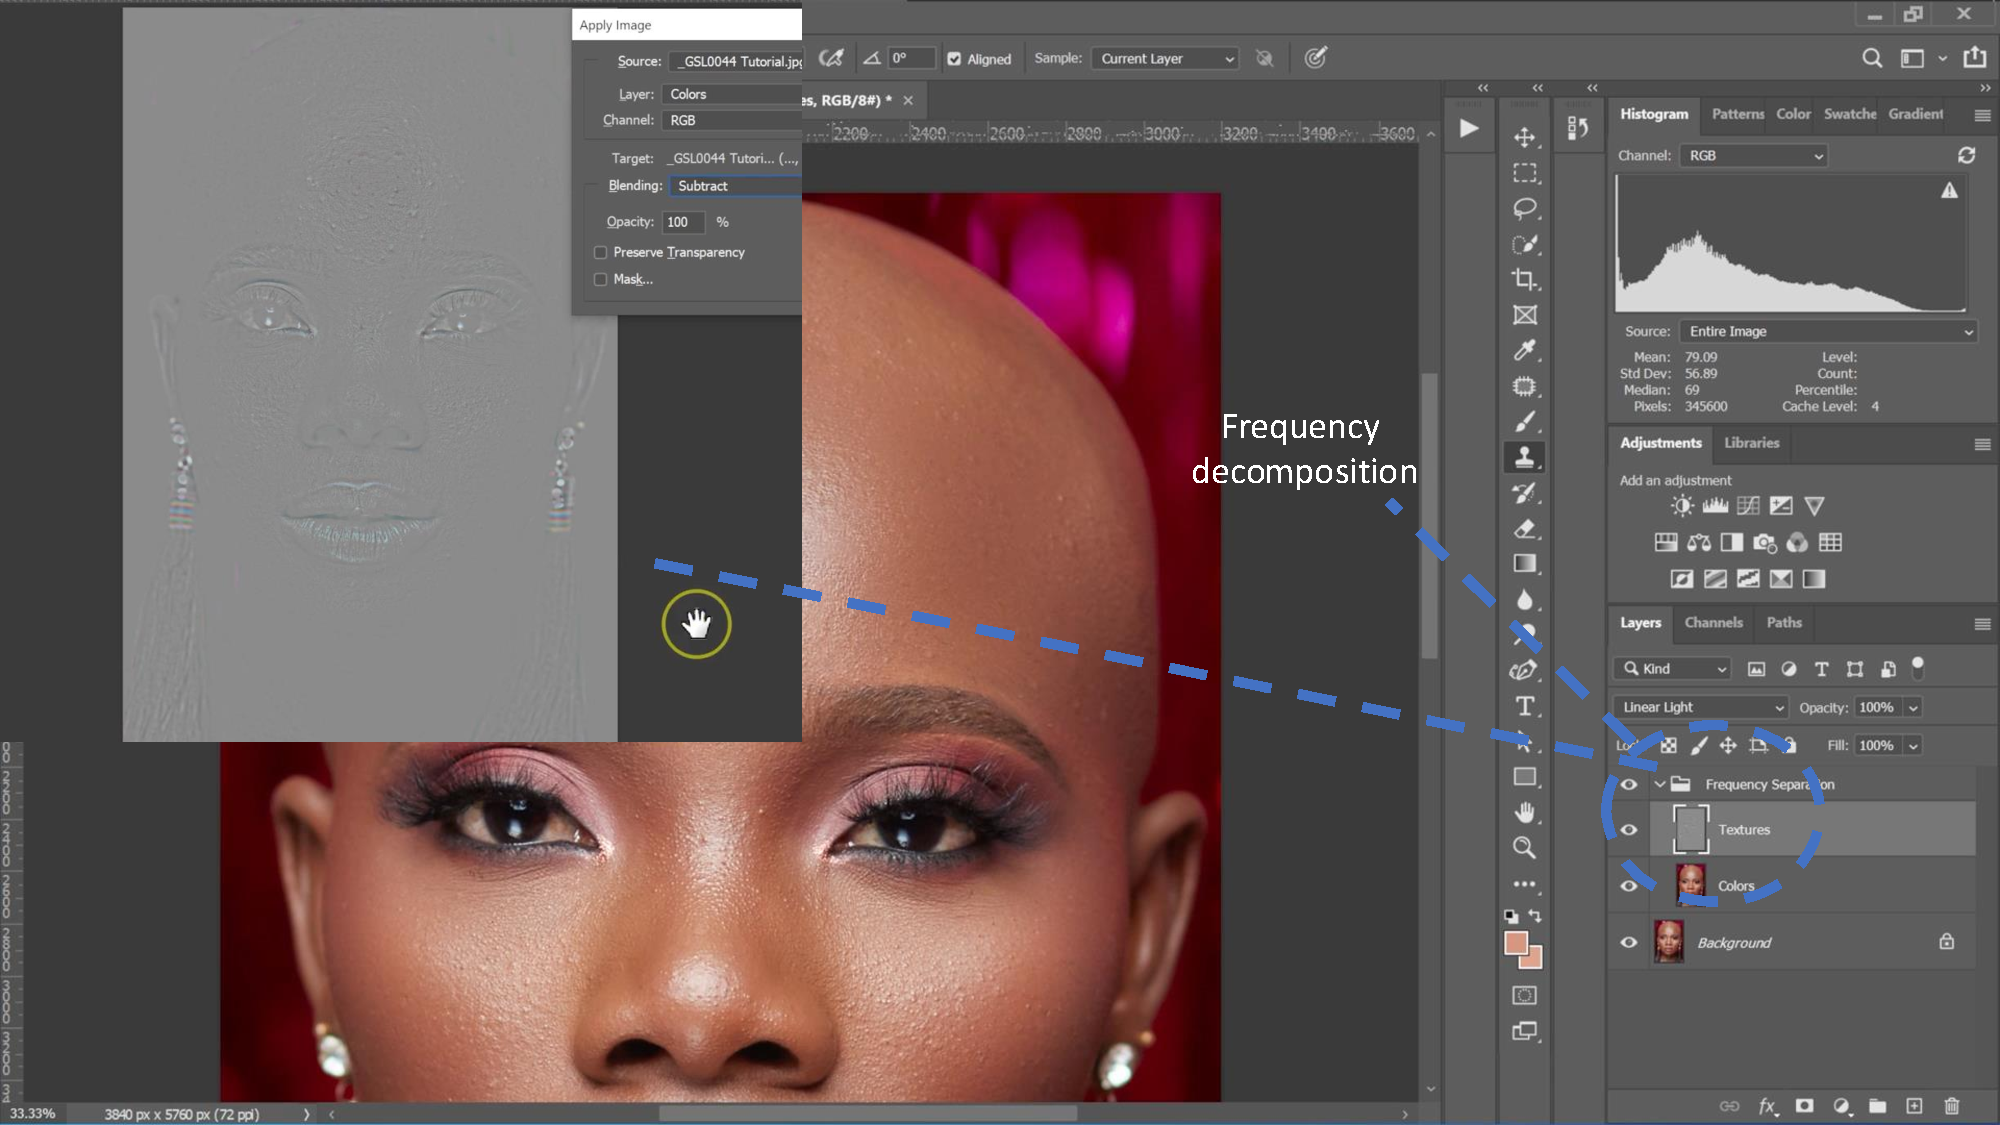
\includegraphics[width=\columnwidth]{Chapters/detail-retouching-figs/PS1.pdf}
    \caption{Frequency decomposition allows artists to have a higher control over different frequency components of an image. Here, the layer shown in the top-left corner is obtained by high-pass filtering of the portrait in the background. Screenshots from [Eustace Kanyanda, 2022].}

\label{fig:PS-high-pass}
\end{figure}

\item Second, image patches of similar content, e.g. skin or hair, are retouched similarly. This means similar patches in the patch space translate into similar edits. The proposed representation leads to a different transformation for patches of differing content. Local filters can offer such edits, where similar contents, such as pores, transform into a similar content, such as a smooth texture:
\begin{figure}[ht]
\centering
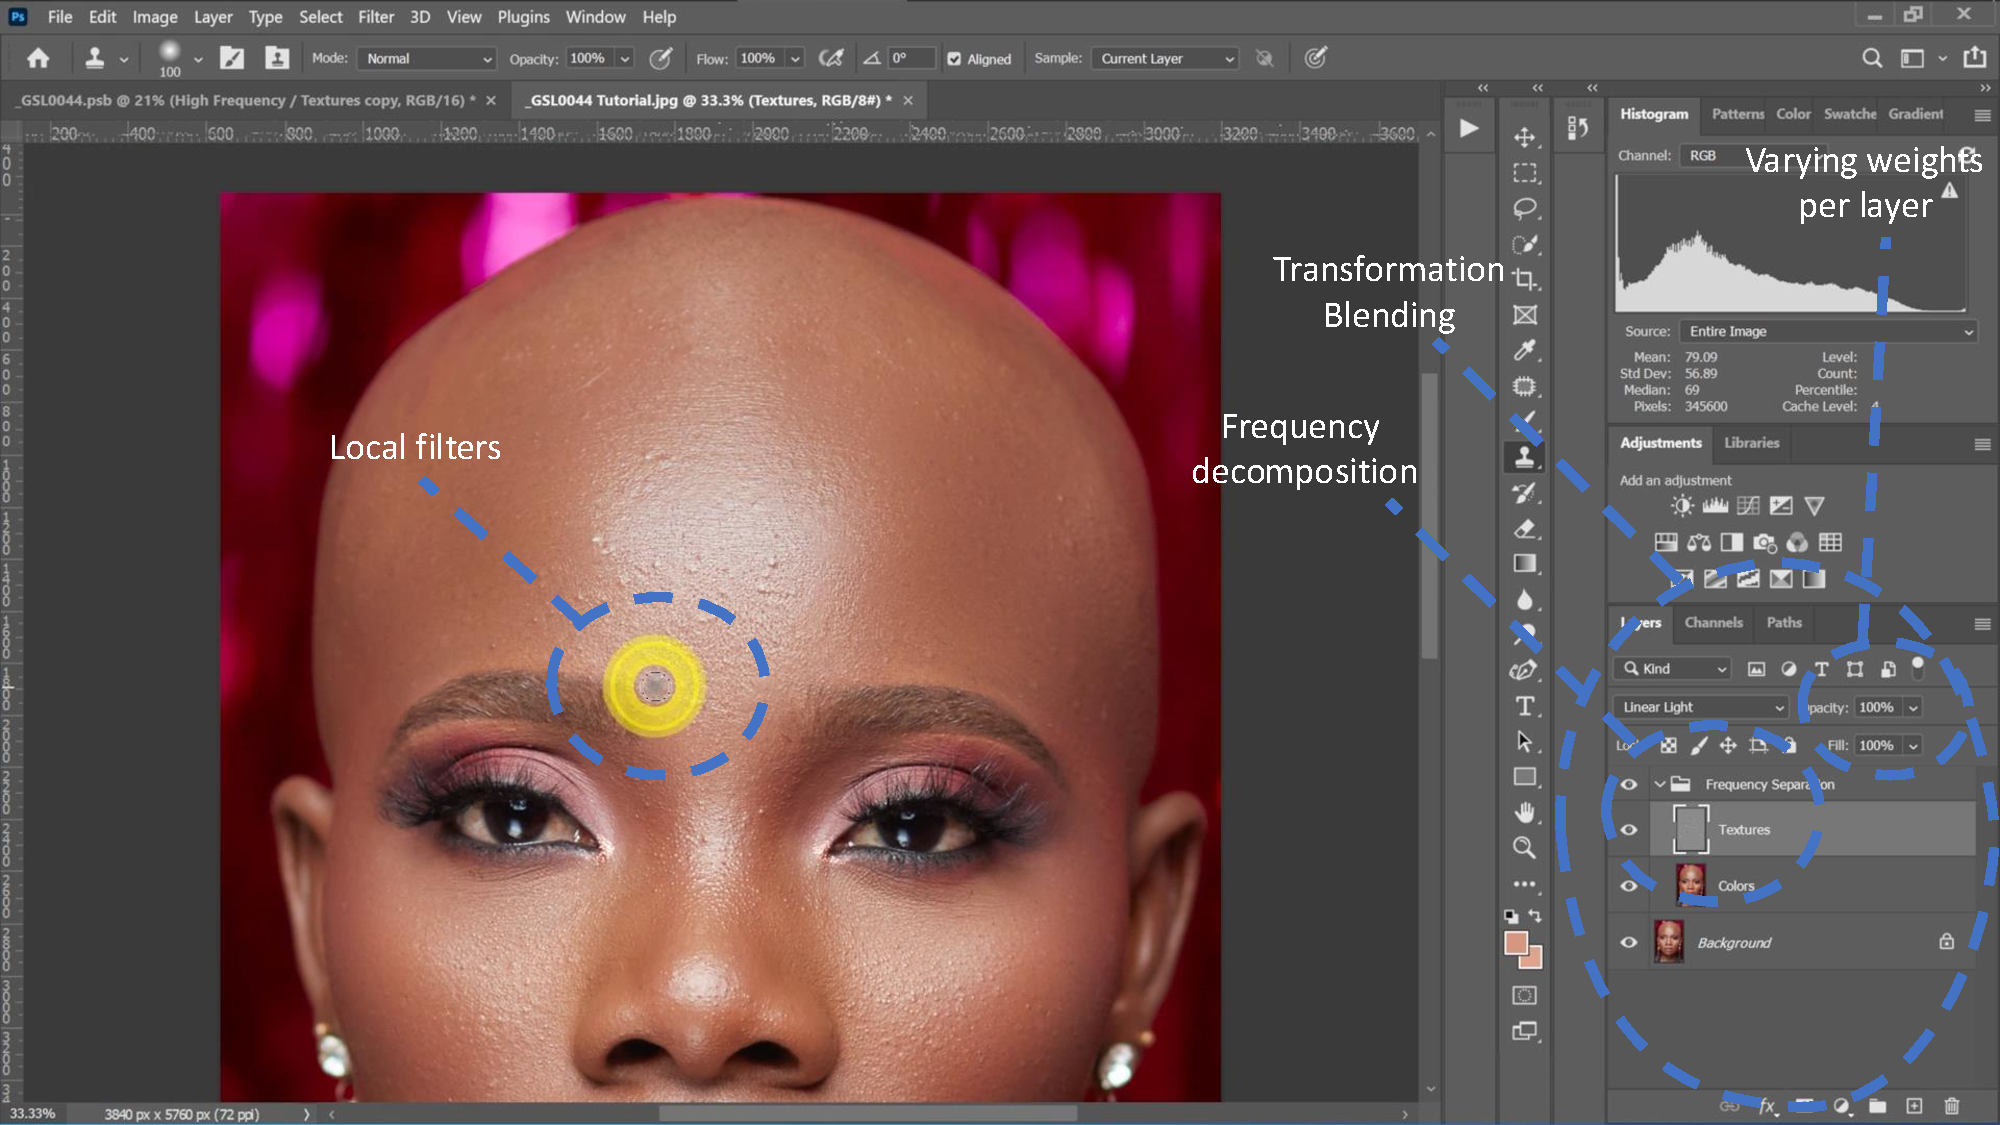
\includegraphics[width=\columnwidth]{Chapters/detail-retouching-figs/PS3.pdf}
    \caption{Local filters, such as brushes, help smoothing the skin by removing the undesired pores on the face. However, it is a tedious task for artists, requiring them to go through each of the visible pores.}

\label{fig:PS-brush}
\end{figure}

\item Third, these edits, global and local adjustments, are typically applied in separate layers and then blended with a subjective opacity value. The neural transformation blending with an MLP block outputting the weights per layer replicates the composition of different layers with their corresponding opacity values:

\begin{figure}[ht]
\centering
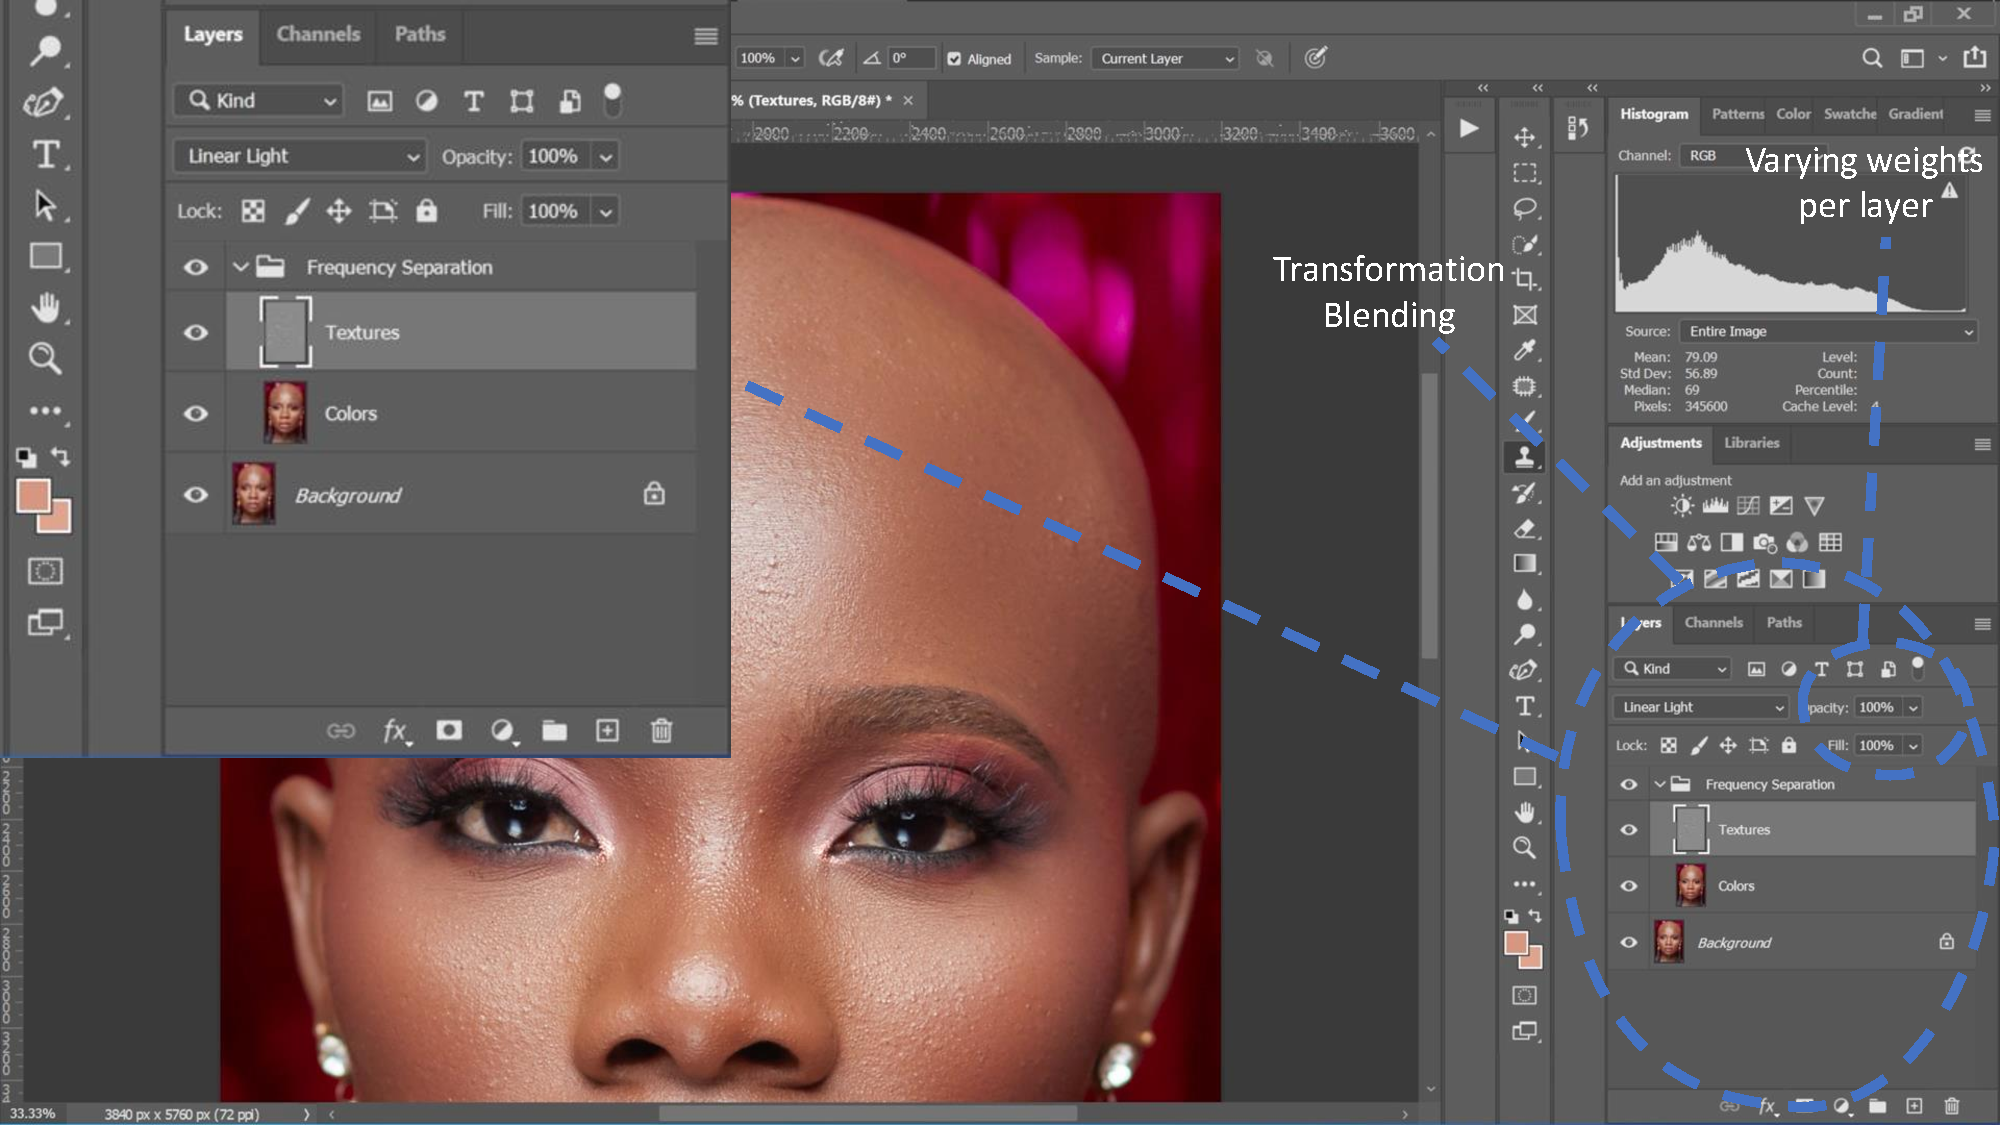
\includegraphics[width=\columnwidth]{Chapters/detail-retouching-figs/PS2.pdf}
    \caption{Artists usually work on separate layers, adjusting varying properties, such as texture, colour, etc. Later, these layers are blended together with their corresponding "opacity" values, shown in the box above the layers.}

\label{fig:PS-all-together}
\end{figure}

\end{itemize}
Although professional artist pipelines inspire this work, I illustrate in the next sections that this new image-to-image mapping representation can replicate the effect of and transfer edits for many filters.



\begin{landscape}\centering
\vspace*{\fill}
\begin{figure}[htpb]
  \centering
  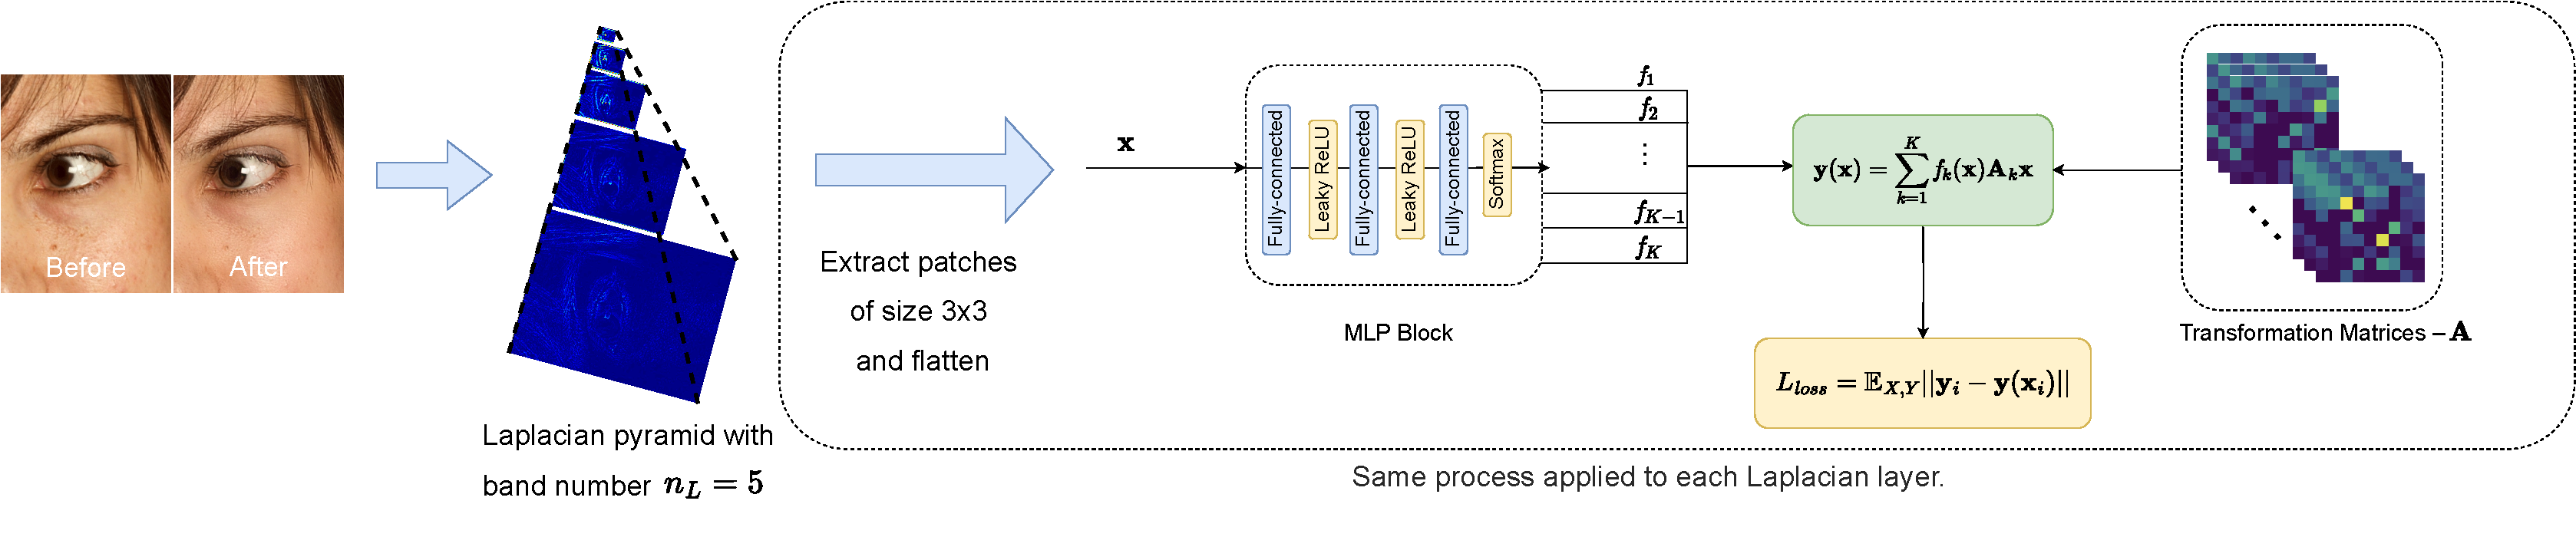
\includegraphics[width=1.5\textwidth]{Chapters/detail-retouching-figs/MainFig.pdf}
  \caption{The proposed technique learns a separate mapping per frequency band by decomposing images into five different bands with a Laplacian pyramid. At each Laplacian band $l$, a separate mapping is defined between flattened patches $\mathbf{x}_i$, $\mathbf{y}_i$ extracted from before-after bands $X_l$, $Y_l$. The field based method (MLP block) adapts transformations to input patches, providing local context-aware adjustments. The transformation matrices and MLP parameters are learned jointly from scratch for each Laplacian band of the before-after pair.}
\end{figure}
\vfill
\end{landscape}


%\begin{landscape}
%\centering
%\begin{figure*}[th] % "[t!]" placement specifier just for this example
%	\centering
%	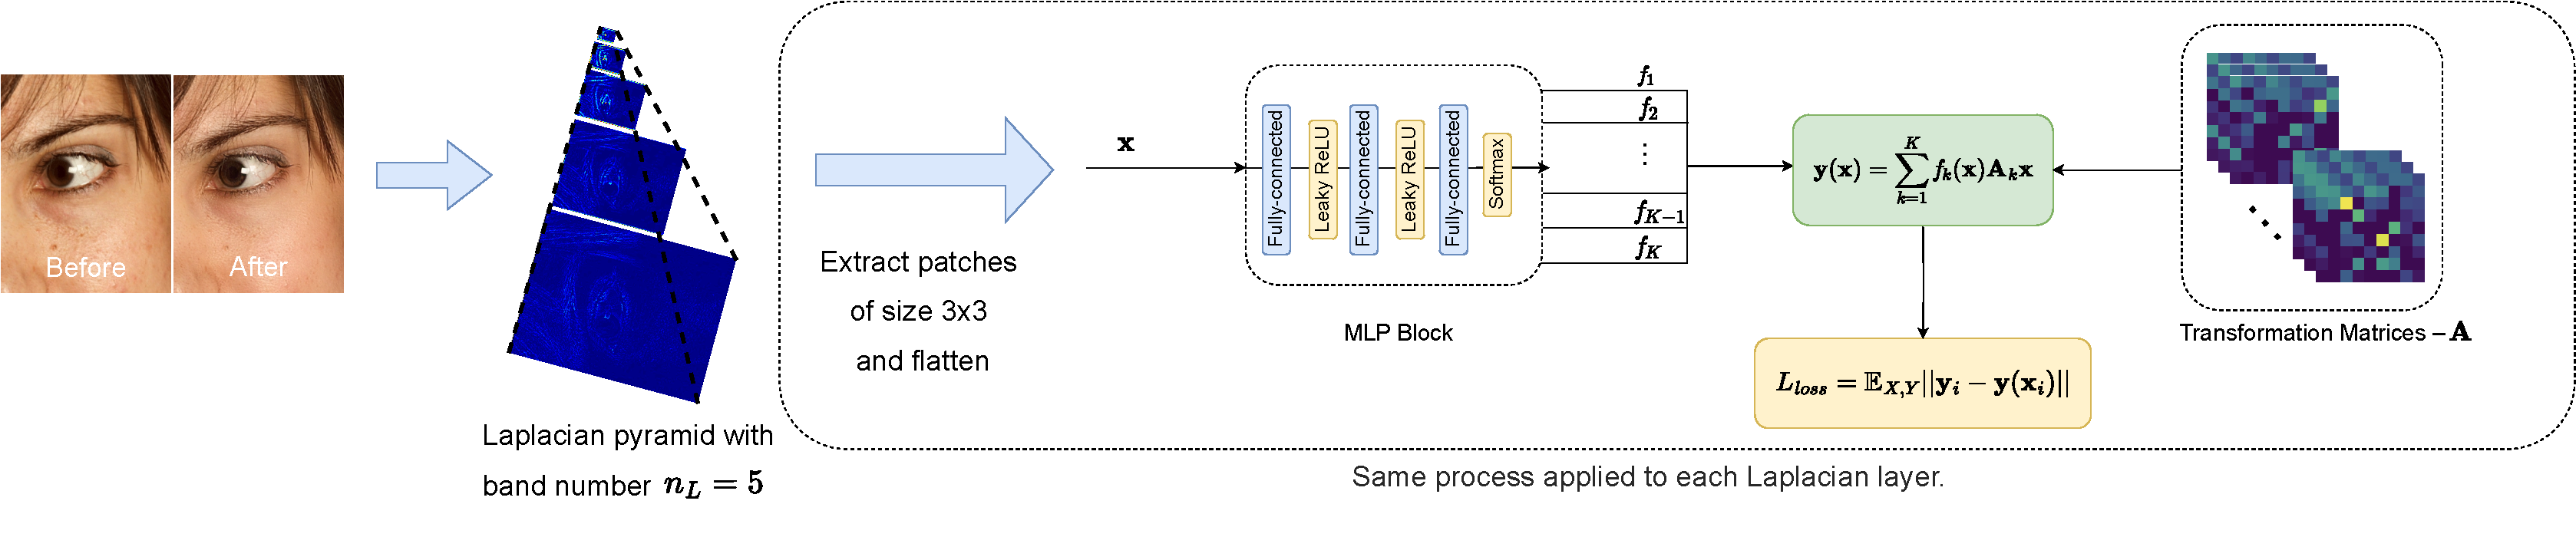
\includegraphics[width=1.5\textwidth]{Chapters/detail-retouching-figs/MainFig.pdf}
    % \includesvg[width=\textwidth]{myfig.svg}
  % \hfill
 %   \caption{The proposed technique learns a separate mapping per frequency band by decomposing images into five different bands with a Laplacian pyramid. At each Laplacian band $l$, a separate mapping is defined between flattened patches $\mathbf{x}_i$, $\mathbf{y}_i$ extracted from before-after bands $X_l$, $Y_l$. The field based method (MLP block) adapts transformations to input patches, providing local context-aware adjustments. The transformation matrices and MLP parameters are learned jointly from scratch for each Laplacian band of the before-after pair.}

%\label{fig:modelT}
%\end{figure*}
% \end{landscape}

\section{One-shot retouching}
\label{sec:Methodology}

\subsection{Frequency decomposition}\label{sec:thePatchMap}
% \myworries{Modify equations in the box - transpose is unnecessary}

I first decompose example and input images into different frequency bands by constructing a Laplacian pyramid to capture details at multiple scales. In principle, it is possible to utilise any multiscale image decomposition method. However, I observed that a basic Laplacian pyramid helped in capturing more accurate and generalisable results compared to a guided or bilateral pyramid. Therefore, I decompose images by

\begin{equation} 
	X_l = L_l(X) = 
 \left \{ \begin{aligned}
        X - G(2) \ast X \hspace{5mm} &l=0\\
        G(2^l) \ast X - G(2^{l+1}) \ast X \hspace{5mm} &l>0,
       \end{aligned}
 \right.
\end{equation}
where $G(\sigma)$ is the normalised Gaussian kernel, and $\ast$ denotes convolution. I also store the low-pass filtered image $S(X)$ such that $X = S(X) + \sum_{l=0}^{n_L} L_l(X)$. I then downsample each $L_l(X)$ and $S(X)$ according to the maximum frequency present at that band. This allows me to use small $3 \times 3$ patches at each band. In the experiments, I used $n_L = 5$ bands for the Laplacian pyramid.


Since each band is processed independently, I explain the steps of our technique below for two generic images $X$ and $Y$.


\subsection{Transformation blending}\label{sec:Blending}

The mapping is defined between patches $\mathbf{x} \in \mathbb{R}^{d_X}$ to $\mathbf{y} \in \mathbb{R}^{d_Y}$ extracted from $X$ and $Y$, respectively, where the patches are denoted by vectors stacking the pixel values, and the patch spaces are defined by $\mathbb{R}^{d_X}$ and  $\mathbb{R}^{d_Y}$. For all results in this work, I work with $3 \times 3$ patches and thus $d_X = d_Y = 9$.

The mapping takes the form of a weighted average of learned transformation matrices $\mathbf{A}$, where each transformation matrix $\mathbf{A}_k$ is first multiplied with its corresponding blending weight: 

\begin{equation} 
	\mathbf{y} (\mathbf{x}) = \sum_{k=1}^K
	\mathit{f}_k (\mathbf{x}) \mathbf{A}_k \mathbf{x},
	\label{eq:weightedSum}
\end{equation} 
Here, $K$ is the number of transformation matrices, and $f_k$ are the blending weights, learned by an MLP block of output size $K$. The $\mathbf{A}_k$'s and $f_k$'s are jointly learned by minimizing the following loss on patches extracted from the before and after images.

\begin{equation}
    L_{loss}  = \mathbb{E}_{X, Y} || \mathbf{y}_i -   \mathbf{y} (\mathbf{x}_i) ||
\end{equation}

Each $\mathbf{A}_k$ corresponds to a different type of transformation and the $f_k(\mathbf{x})$'s, represented with the MLP, allow for a smooth transition between different transformations. The form of $f_k$'s is relatively simple with three fully-connected layers and nonlinear activation functions applied after each layer. This blending forms a simple but expressive transformation as illustrated in Section \ref{sec:results}.

\subsection{Retouching an input image}

I process the input image $I$ the same way as the before-after pair. First, I decompose the input into its Laplacian layers and then extract patches for each layer. After applying the learned mappings $M_l$ to the patches of the corresponding layers $L_{l}(I)$ independently, I then reconstruct the Laplacian bands of the output image $O_l$ by placing the patches in their spatial locations and averaging over the overlapping regions. Later, I obtain the final output image $O$ by summing the outputs $O_l$ and the residual of the input image:
\begin{equation}
    O = S(I) + \sum_{l=0}^{n_L} M_l(L_l(I))\,.
\end{equation}




\subsection{Implementation}
\label{sec:Implementation}

\paragraph{Patch size and stride.} In order to capture each frequency band at the right level of detail, I do not upsample the images $L_l(X)$ and use a small $3 \times 3$ patch size (with stride $1$). I experimented with larger patch sizes. However, this turned out to be counterproductive for the detail levelItarget, as details are blurred in larger patches. They also led to overfitting and were, in general, harder to optimise for. I used a stride of $1$, and hence patches overlap on the image plane. The overlapping patches are averaged while reconstructing the image.

\paragraph{Detail and colour modifications.} This work aims to capture intricate details present in highly detailed retouches and a wide range of image processing operators. Based on the observation that various operators can edit materials in the image space using the luminance component~\cite{Boyadzhiev15Band}, I focus on learning changes in luminance while preserving the input chrominance channels. 

\paragraph{Evaluation metrics.} To quantitatively compare the technique with state-of-the-art methods, I used PSNR and SSIM metrics. This is only possible if the before-after image pair was processed with a known, reproducible operator (see Section~\ref{sec:Comparisons} for details).


\paragraph{Training details.}\label{train_det} I train different mappings with the same structure, defined in Equation \ref{eq:weightedSum}, for each frequency band of the Laplacian pyramid. Each mapping consists of one MLP block and $K$ number of transformation matrices, which are learned jointly per frequency band from scratch for each before-after pair. The MLP block employed in the experiments consists of three fully-connected layers and non-linearities applied after each layer. The output size of the last layer is the same as the number of transformation matrices.

To normalize the weights, I choose the last activation function to be Softmax, while for the first two layers, I apply Leaky ReLU. Each transformation matrix is randomly initialised with the uniform distribution in the range of $[0, 1]$. All experiments use the Adam optimiser with a learning rate of $10^{-2}$, which exponentially decays with a decay rate of $0.96$. I use $l_1$ loss function in all experiments. Through backpropagation, both the MLP parameters and the entries of the transformation matrices are jointly learned. The pseudocode for both the training and inference procedures are the following:

\begin{algorithm}
\caption{One-shot Detail Retouching}
\SetKwFunction{FDetailRetouch}{Train}
\SetKwFunction{FPyramid}{LaplacianPyramid}
\SetKwFunction{FMLPBLOCK}{MLPBlock}
\SetKwFunction{FPatch}{ExtractPatch}
\SetKwFunction{Fprob}{Backpropagate}
\SetKwProg{Fn}{Function}{:}{}
\Fn{\FDetailRetouch{'before' image $X$, 'after' image $Y$}}{
	\Comment{Decompose images into its Laplacian bands.}\\
        $X_l \gets \FPyramid(X)$\;
        $Y_l \gets \FPyramid(Y)$\;
        
        \For{$l \gets 0$ \KwTo $n_l$}{
        \Comment{Extract patches from the images.}\\
        $x_i \gets \FPatch(X_l)$\;
        $y_i \gets \FPatch(Y_l)$\;
        $f_k \gets \FMLPBLOCK(x_i)$\;
        $y(x_i) \gets \sum^{K}_{k = 0} f_k(x_i) A_k x_i$\;
        $\mathcal{L} \gets E_{X, Y} \abs{(y(x_i) - y_i)}$\;  
        $(f_k, A_k) \gets \Fprob(\mathcal{L})$}
        }
\end{algorithm}

\begin{algorithm}
\caption{One-shot Detail Retouching}
\SetKwFunction{FDetailRetouch}{Inference}
\SetKwFunction{FPyramid}{LaplacianPyramid}
\SetKwFunction{FMLPBLOCK}{MLPBlock}
\SetKwFunction{FPatch}{ExtractPatch}
\SetKwFunction{Fpatchmerge}{MergePatch}
\SetKwProg{Fn}{Function}{:}{}
\Fn{\FDetailRetouch{input image $I$, blending weights $f_k$, transformation matrices $A_k$}}{

        $I_l \gets \FPyramid(I)$\;
        
        \For{$l \gets 0$ \KwTo $n_l$}{
        $i_i \gets \FPatch(I_l)$\;
        \Comment{Transform input patches $i_i$ with learned weights and matrices.}\\
        $o_i \gets \sum^{K}_{k = 1} f_k(i_i) A_k i_i$\;
        	\Comment{Place the patches on the output grid $O_l$.}\\
        $O_l \gets \Fpatchmerge(o_i)$}
     
        \Comment{Sum all output bands with input residual.}\\
        $O = I_{n_l} + \sum_l O_l$\;
        \Return $O$}
        
\end{algorithm}

\section{Results}
\label{sec:results}


\subsection{Ablation Studies}\label{ablation}
The success of the learned mappings relies on two key components: patch-adaptive retouching and transformation blending. I thus conduct experiments to illustrate the significance of these.

%Ifirst investigate the effect of the number of transformation matrices, $K$. 
% \paragraph*{Transformation Matrices.}
\paragraph{Transformation Matrices.} I compared transformation matrices of size $9 \times 9$ with scalar values. The method still remained spatially-varying, since I left the MLP the same, and used $K=256$ scalar weights. I tested both methods on 100 images and computed average PSNR values. I observed that the technique with matrices performed better than scalar values even in simple algorithmic filters, such as Gaussian and Unsharping Masking (around 2 dB and 3 dB higher PSNRs, respectively). 

As the complexity of a retouching style depends on multiple factors, such as artists’ design choices, user preferences, or the artist toolbox, it is challenging to analyse such effects on retouching examples quantitatively. For simple algorithmic filters, such as a Gaussian filter or unsharp masking, $K=1$ can sufficiently reproduce the filter. In contrast, more complex algorithms, such as a bilateral filter, require more matrices to capture the algorithmic edits accurately (Figure \ref{fig:ablation_K}). Since retouching edits combine the effect of multiple operators and are highly non-linear, I empirically found $K=256$ offers effective results for the retouching examples. 

\begin{figure}[th] % "[t!]" placement specifier just for this example
    \centering
	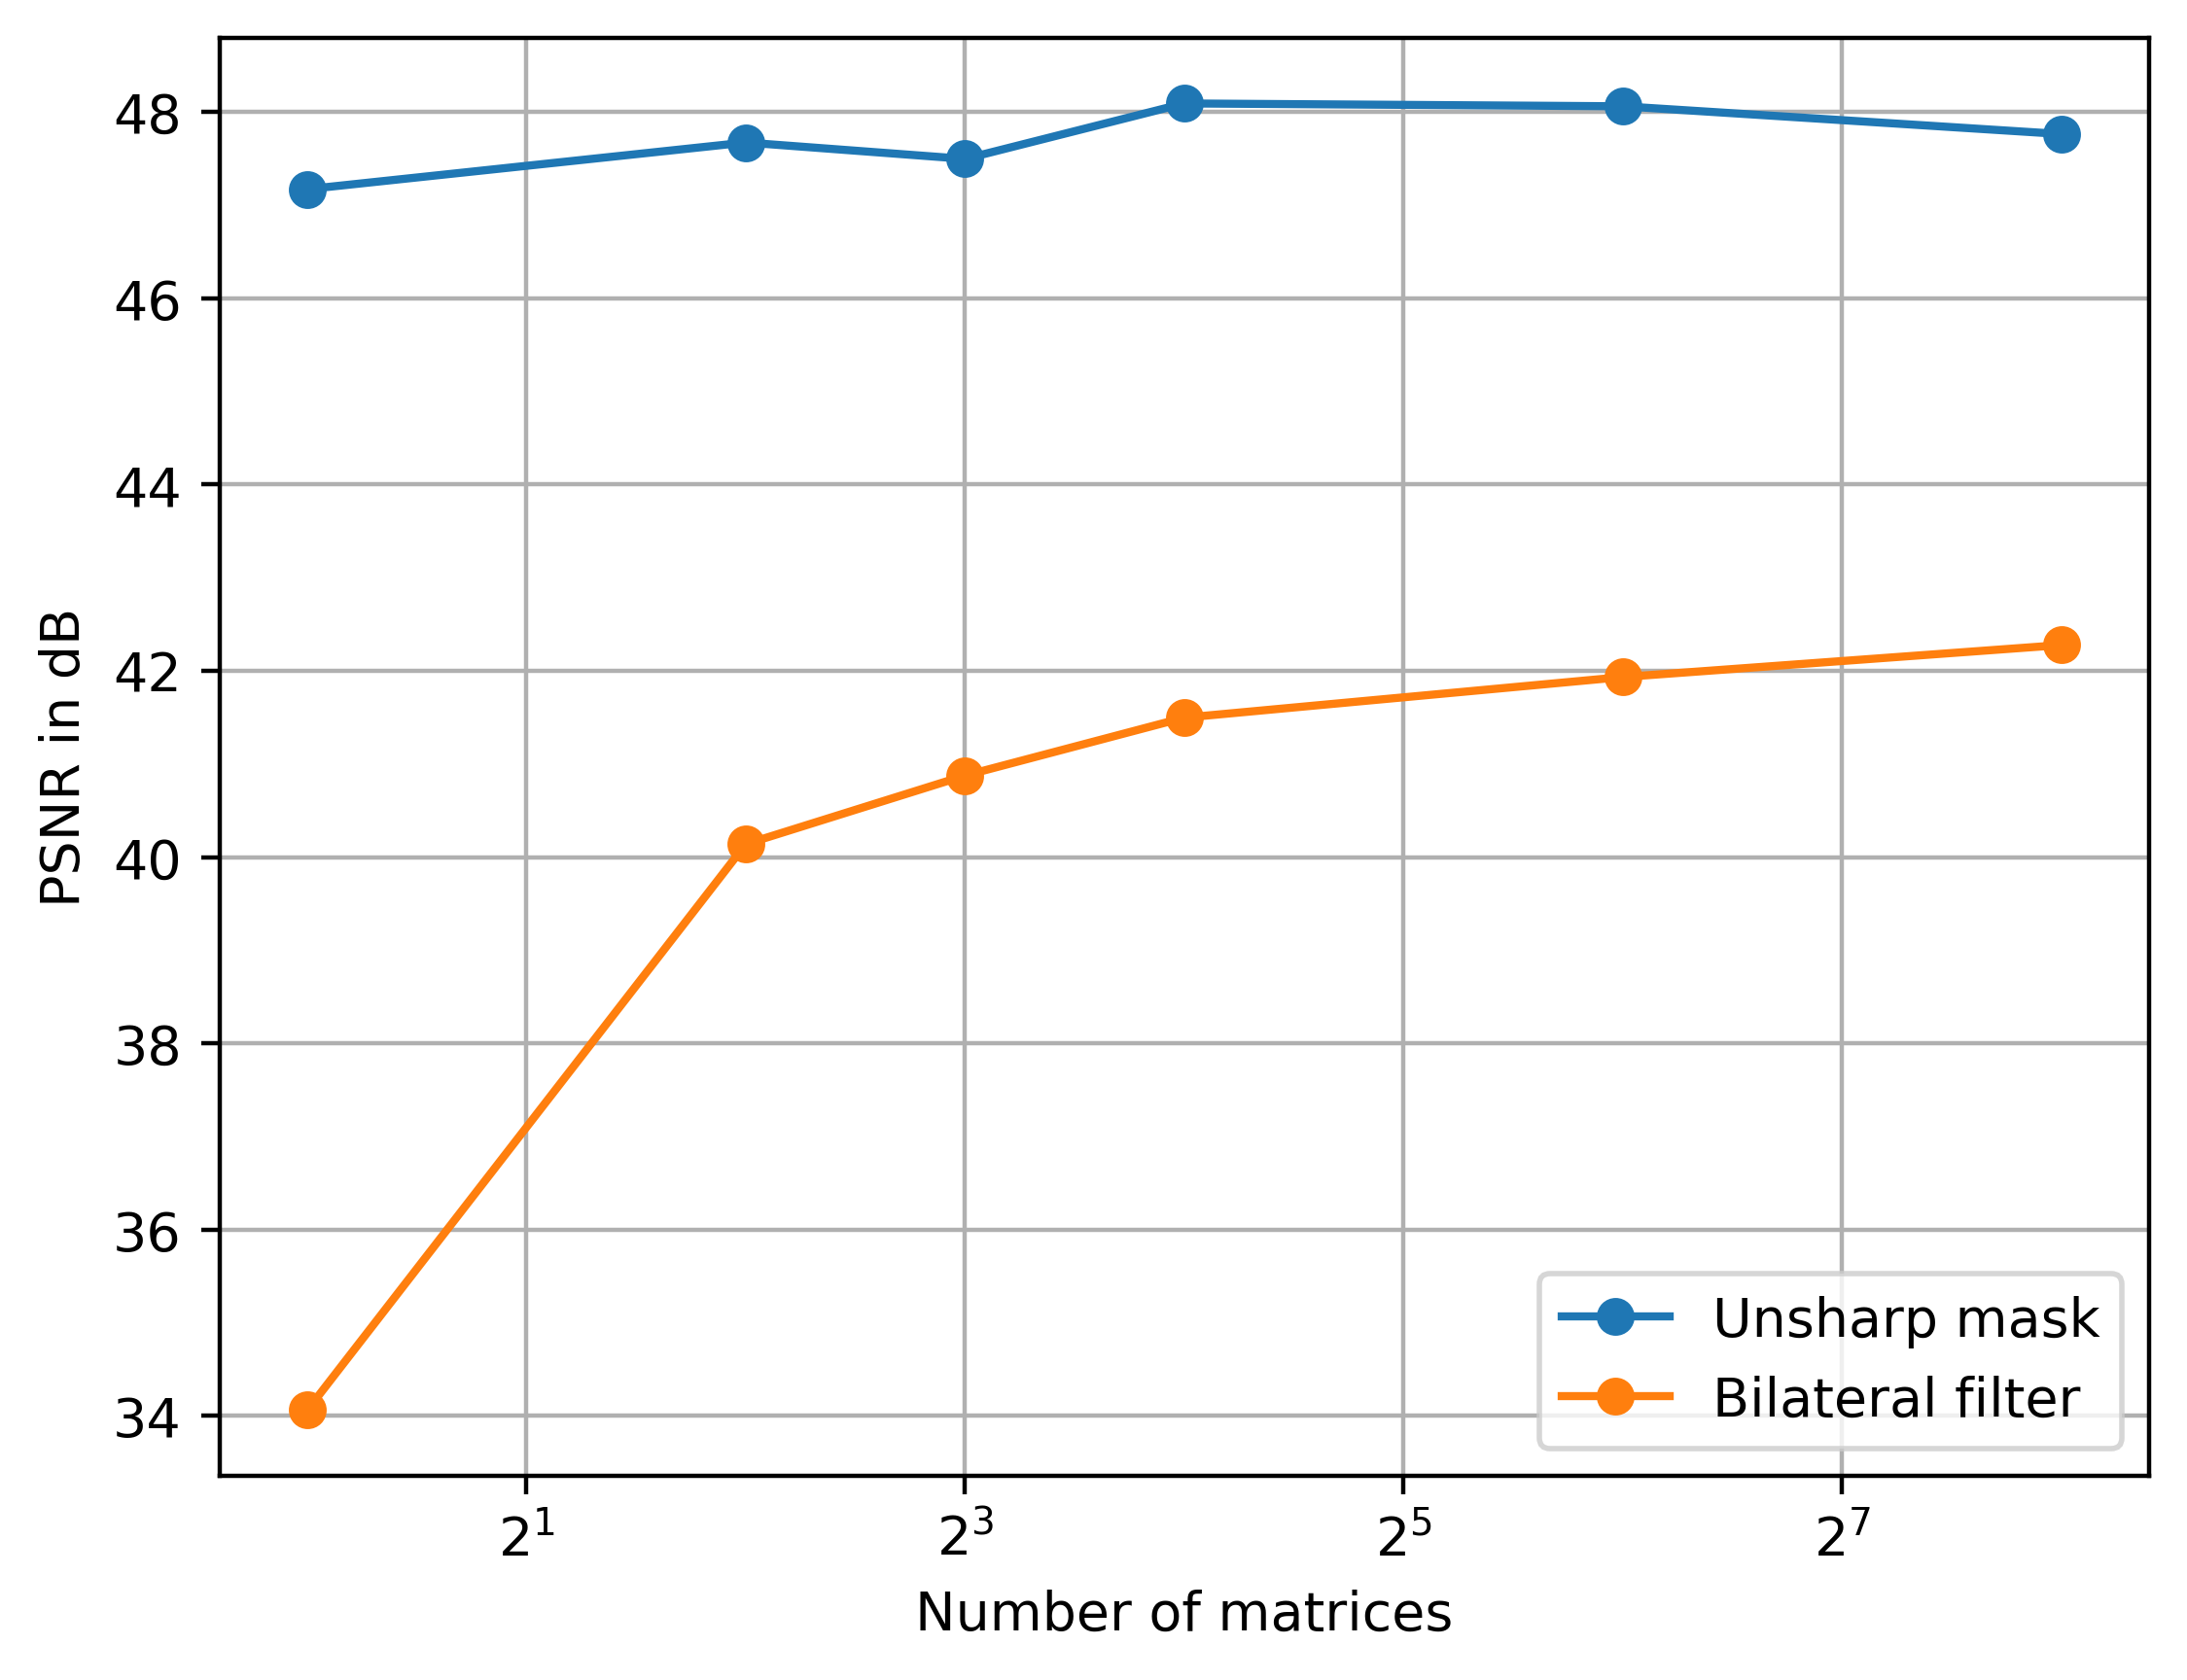
\includegraphics[width=0.5\columnwidth]{Chapters/detail-retouching-figs/ablation_matrices.png}

    \caption{The higher the complexity of the learned algorithm, the more transformation matrices the technique requires to capture the effects on local regions accurately. While $K=1$ can be sufficient for the model to capture unsharp masking, it requires more matrices to represent bilateral filtering precisely.}

    \label{fig:ablation_K}
\end{figure}

\begin{figure}%[H]
\centering
\includegraphics[width=0.8\columnwidth]{Chapters/detail-retouching-figs/AblationStudy_K.pdf}
    \caption{An MLP regressor cannot capture local edits, resulting in inaccurate retouching edits, such as blurring on the skin or around the eyes.}

\label{fig:ablation_MLP}
\end{figure}
% \paragraph*{Patch-adaptive Transformation Blending.}
\paragraph{Patch-adaptive Transformation Blending.} I also compared the patch-adaptive mapping to an MLP regressor on the extracted patches. This directly learns the mapping from the decomposition of example before-after images instead of utilising blended transformations. The MLP regressor follows a similar architecture as the MLP block (Figure \ref{fig:modelT}), with the only difference being the last activation function. I used Leaky ReLU here, since the Softmax function outputs pseudo-probabilities and is unsuitable for regression. Not explicitly handling the spatially-varying structure of the mapping and directly regressing limits the expressiveness of the model. This results in blurry results as shown in Figure~\ref{fig:ablation_MLP} because such a model cannot capture edits in intricate details, such as highlights around eyes and hair or brightening of the skin. I also tried increasing the capacity of the MLP regressor but did not observe much improvement in performance.


\paragraph{Weights visualisation.} To study the effectiveness of the weights across an image, I randomly chose eight transformation matrices and reconstructed their corresponding weights per Laplacian band. The reconstruction occurs in the same way as image patches, being placed in their location. However, since each patch of size $3 x 3$ has only one weight,Ido not need to take average over overlapping areas. Also, cropped the last eight columns of the reconstructed weight images since they were all zeros due to the size difference with patches. Figure \ref{fig:weight-vis} shows eight different reconstructed weights for each Laplacian band, obtained by the model trained with the example images in the teaser (middle \& right insets). The input to the model and the output retouched image are shown on top. As can be seen, the weights have varying values around different regions across the bands. Note that the resolution of the bands is increased to the same size for better visualisation. Otherwise, during training, each band’s resolution is kept its size based on the Laplacian pyramid.

\begin{figure}%[H]
\centering
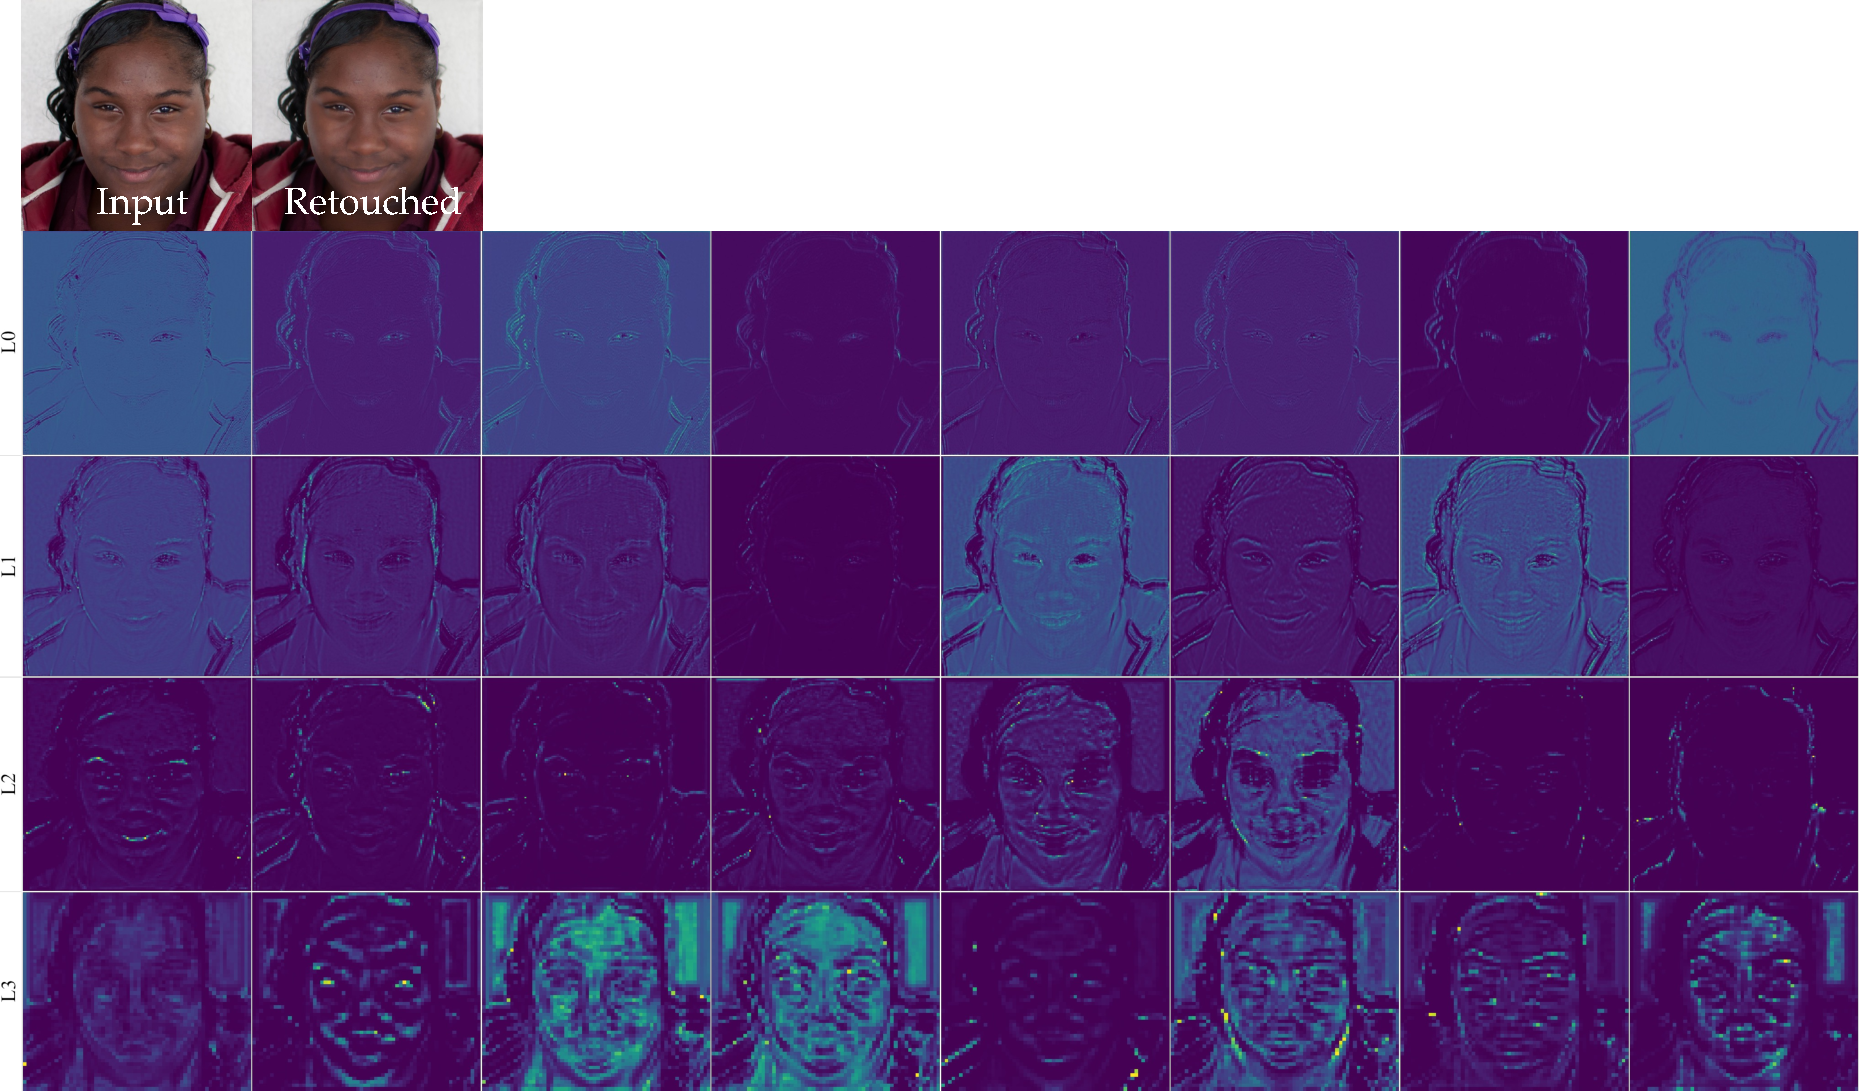
\includegraphics[width=0.8\columnwidth]{Chapters/detail-retouching-figs/weight_visualise.pdf}
    \caption{Visualisation of the reconstructed patch-adaptive weights of the model trained with example images in the teaser. Here, the input to the model is shown on top, and each row shows the weights in the corresponding Laplacian band, indicated on the left.}

\label{fig:weight-vis}
\end{figure}

\subsection{Qualitative Results}
I tested the proposed technique on a diverse range of before-after pairs, including face images from the \textbf{FFHQ} dataset \cite{karras2019style}.I focus on human portraits and face retouching in the experiments as they are arguably the most common and prioritised types of photos for retouching.I also illustrate that the technique provides visually pleasing results in different types of images, such as materials or rooms, and accurately captures image processing filters.

\begin{figure}[th] % "[t!]" placement specifier just for this example
    \centering
	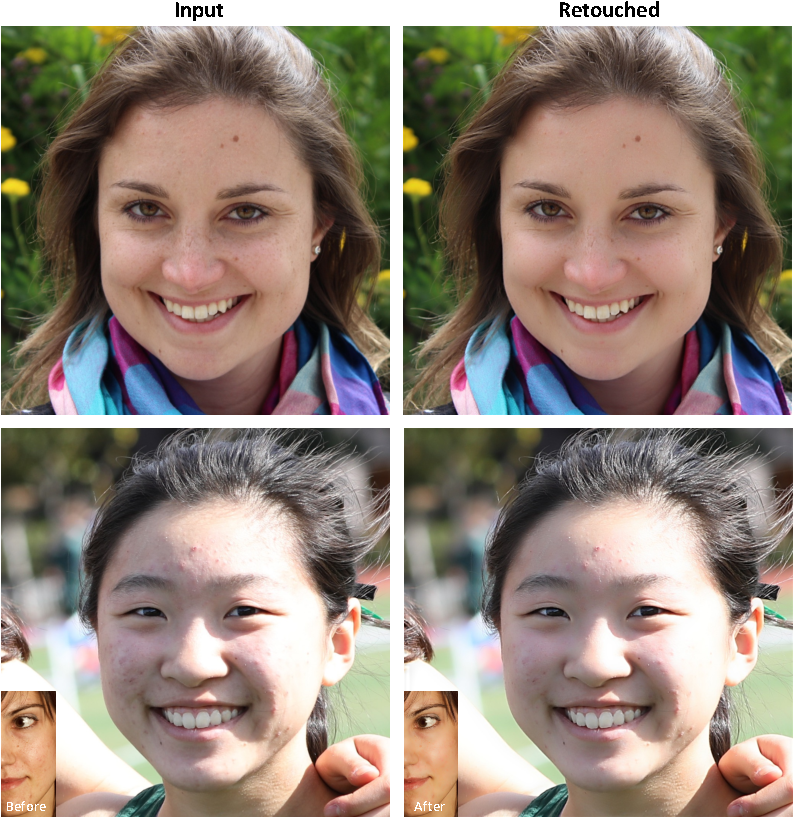
\includegraphics[width=0.8\columnwidth]{Chapters/detail-retouching-figs/res_diff_light_2_cvmp.pdf}
    \caption{\label{fig:newdataset_ex}The reproduced retouching style from the example pair (inset) improves skin texture without affecting fine details, such as eyes and hair, for a visually improved portrait. Moreover, the technique generalises well to faces with different lighting conditions and accurately reproduces the example retouching style.}
 
\end{figure}
% \paragraph*{Face retouching - skin and eye filters:}\label{faceretouching}
Human faces pose a particular challenge for the one-shot setting. However, the model can still capture highly nonlinear retouching edits and generalises well to different types of faces, view directions, and lighting conditions, as illustrated in Figures~\ref{fig:teaser}, ~\ref{fig:newdataset_ex}, and ~\ref{fig:retouchingstyles}.

\begin{figure}[th] % "[t!]" placement specifier just for this example
	\centering
	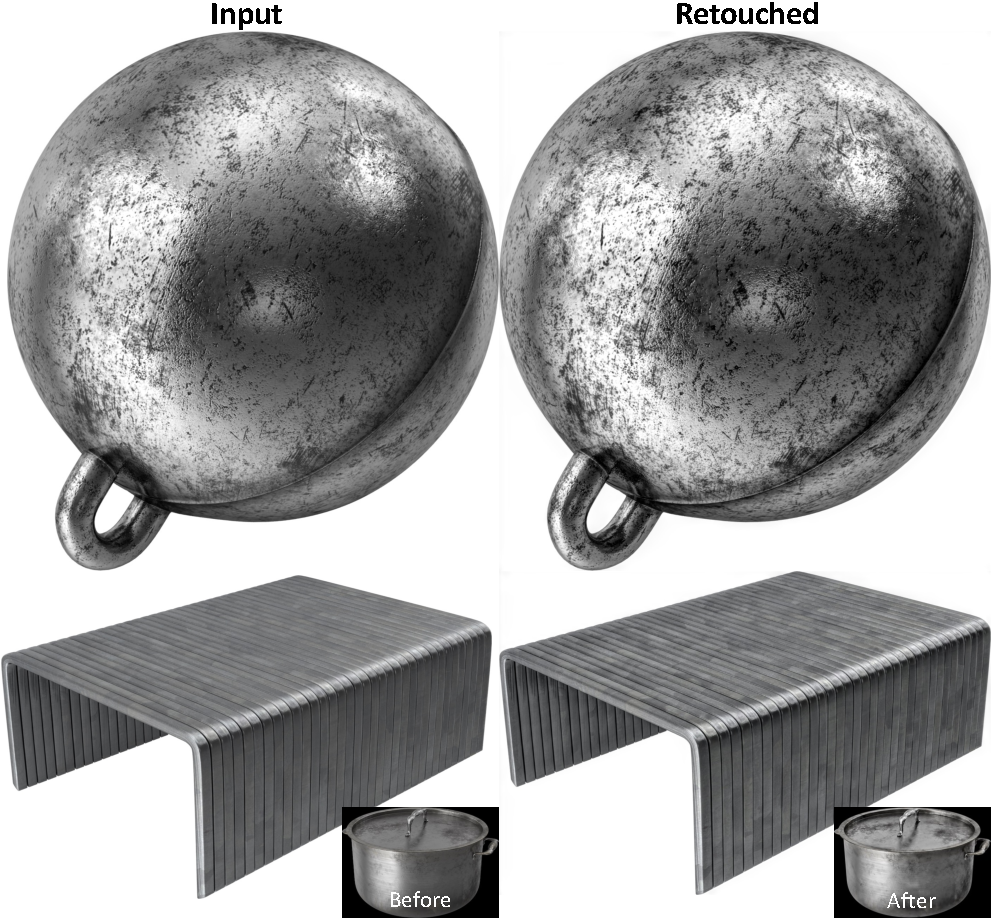
\includegraphics[width=0.8\columnwidth]{Chapters/detail-retouching-figs/MaterialResults.pdf}
    \caption{\label{fig:material_res}Material editing results on photos (left), and rendered images (right), based on the before-after pair (inset). The details, such as scratches or lines are emphasised, and materials became shinier. Image courtesy of royalmix (top and bottom-inset), tsmdunn (bottom). (PixelSquid).}

\end{figure}

The example pairs in Figures~\ref{fig:teaser}, ~\ref{fig:newdataset_ex}  and ~\ref{fig:retouchingstyles} were generated by brushing onto the skin with artist created brushes, eye sharpening (sharpening example in Figure~\ref{fig:teaser}), and further brightness/contrast adjustments. These brushes first decompose the skin into a detail and base layer, typically with frequency decomposition, alter the detail layer and blend it with the base layer. They differ in how (1) they decompose the skin into the layers, i.e., what frequencies are in each layer, and (2) they edit and blend each layer with different opacity values. This variation creates retouching nuances, as shown in Figure~\ref{fig:retouchingstyles}. The framework can still accurately capture such slight differences in styles. 

\begin{figure}[th] % "[t!]" placement specifier just for this example
    \centering
	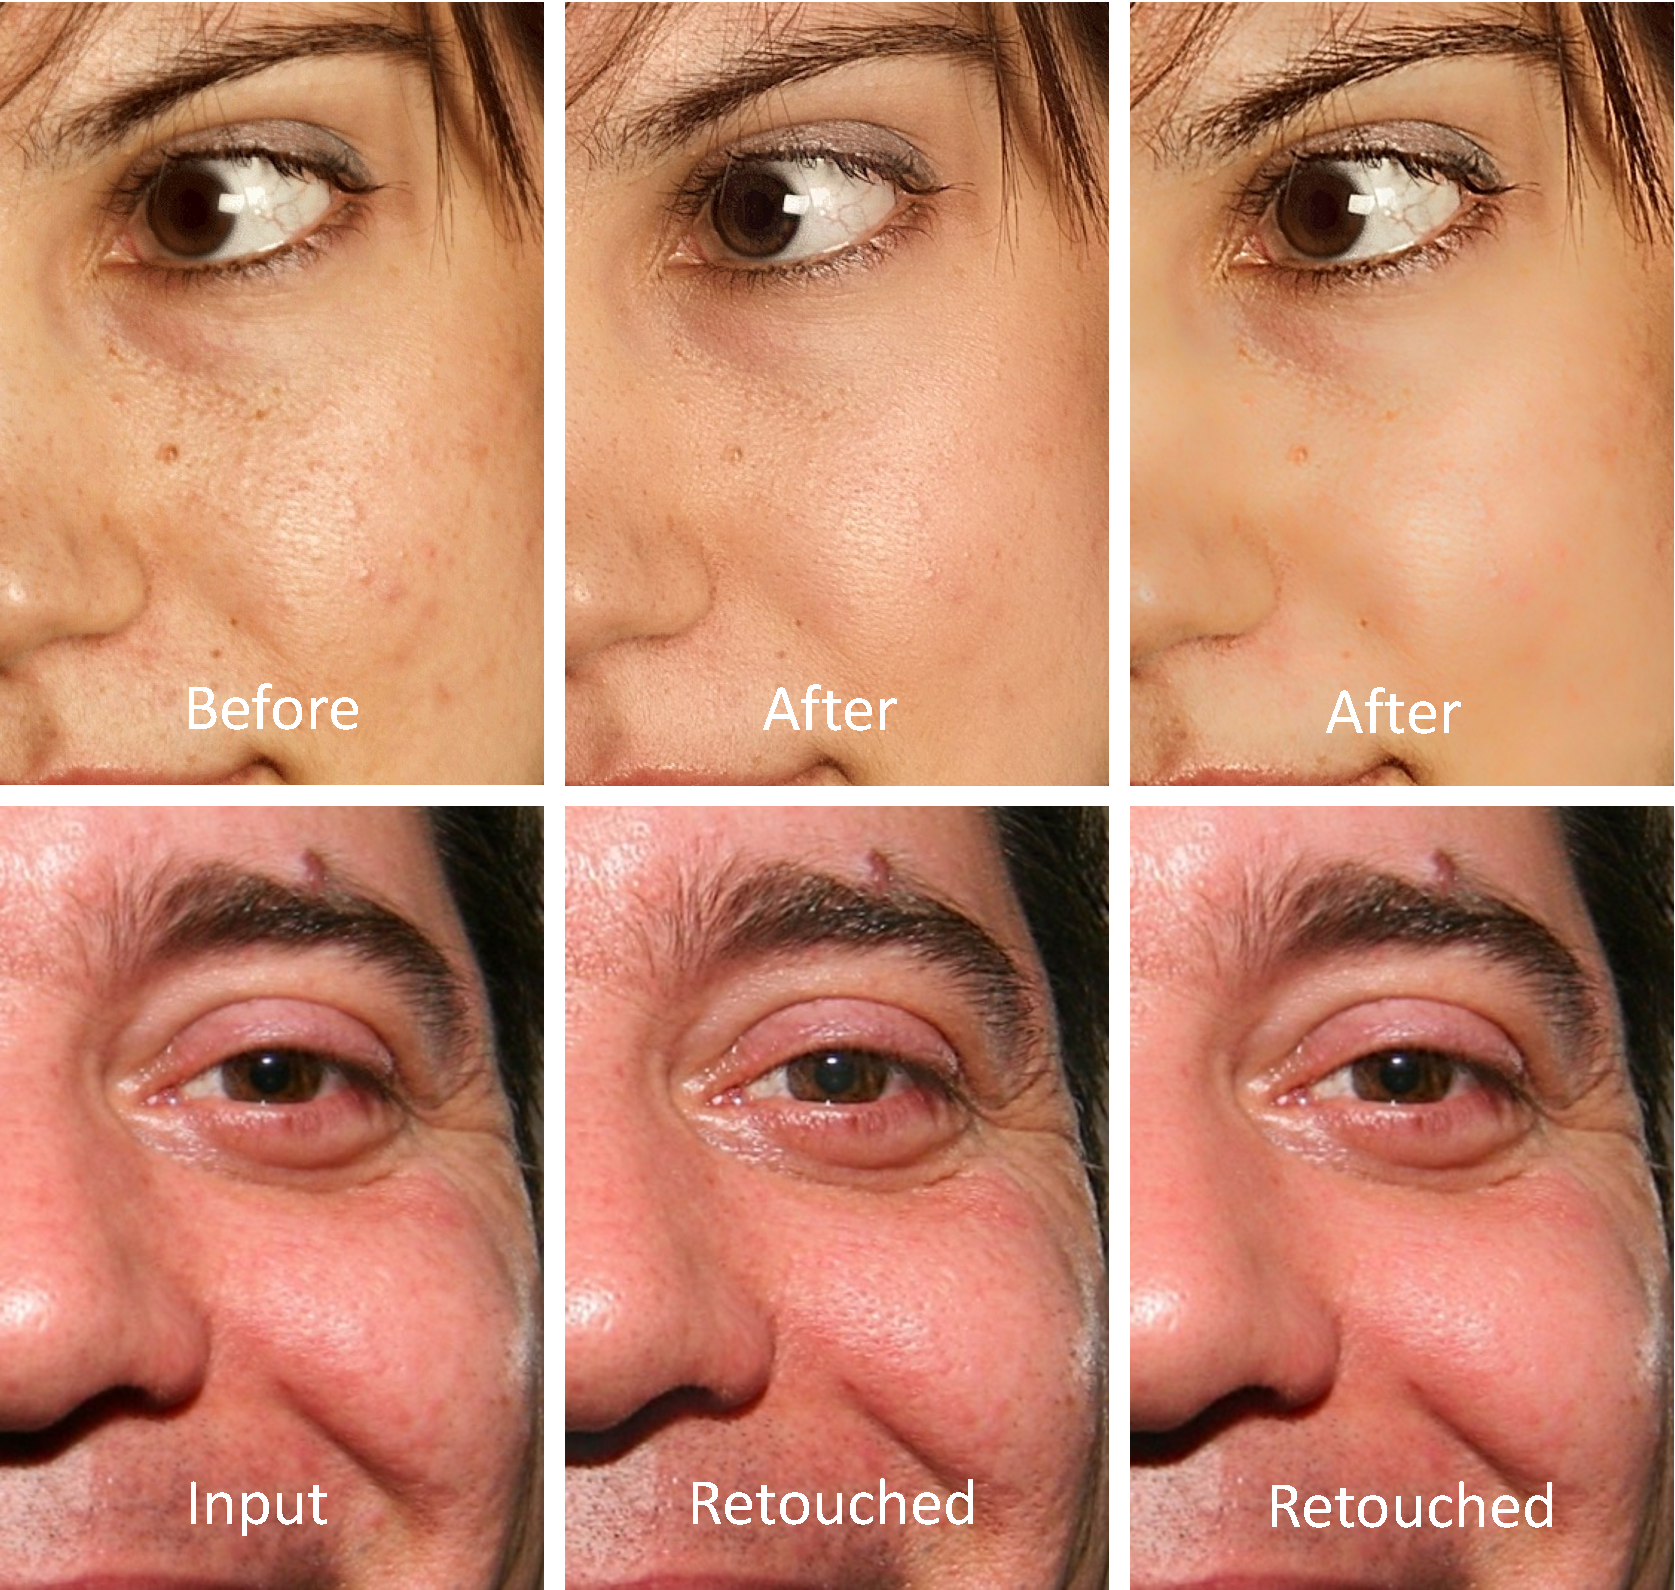
\includegraphics[width=0.8\columnwidth]{Chapters/detail-retouching-figs/Nuances.pdf}
  % \hfill
    \caption{Our patch-adaptive technique can accurately capture the nuances between different
    retouching styles as given by the examples (top row).}
\label{fig:retouchingstyles}
\end{figure}

In all experiments, intricate details of the desired retouching, such as small-scale texture, eye, facial hair or material details, and global features, such as overall lighting and tone, are accurately reproduced. It is interesting to observe that the \emph{glamour} implied by, e.g., the example retouching in Figure~\ref{fig:newdataset_ex} is transferred from the example pair very accurately without causing an artificial look. Zooming into the skin reveals that pores and wrinkles are minimised, and the blemishes and discolouring of the skin are eliminated. At the same time, depending on the retouching edit, details, such as eyes or material texture, are more highlighted or preserved, and delicate features such as hair are preserved well (Figures ~\ref{fig:newdataset_ex}, ~\ref{fig:material_res} and ~\ref{fig:retouchingstyles}). 


In summary, the proposed technique efficiently edits such intricate details, due to the significantly distinct local statistics of the texture at multiple scales, without affecting overlaying structures thanks to its spatially-varying nature and frequency decomposition. 

\subsection{Comparison with the state-of-the-art}
\label{sec:Comparisons}


Although there are various works related to automatic photo enhancement, to the best of our knowledge, none of them works with a single example pair for detail retouching. Therefore, I compare the results with closely related automatic image-to-image translation methods, namely U-Net \cite{ronneberger2015u}, ASAPNet generator \cite{shaham2021spatially}, and Deep edge-aware filters \cite{xu2015deep}. 

I trained each network from scratch with one \textit{before-after} pair. To train the U-Net architecture, I changed the activation function of its last layer to ReLU and used $l_1$ loss function with Adam optimiser (same as ours). Similar to the proposed method, ASAPNet is also a spatially-adaptive network. However, it is instead designed to hallucinate new details. Therefore, I trained their generator model in a similar fashion with $l1$ loss, removing the discriminator. After observing that bilinear downsampling in their model causes checkerboard artifacts, I removed this operator and learned an MLP per pixel, which caused the model to be highly complex with too many parameters. 


\begin{table*}[th]
\centering
\caption{Quantitative performance comparison for the reproduction of various image processing filters. Average PSNR and SSIM values are computed over 182 images of different types of images including faces, landscapes, materials, and rooms. Qualitative results can be found in the supplementary material.We highlight \colorbox{blue!25}{best PSNR} and \colorbox{orange!25}{best SSIM} results.}


\resizebox{\textwidth}{!}{\begin{tabular}{l@{\hskip 0.2in}c@{\hskip 0.1in}c@{\hskip 0.1in}c@{\hskip 0.1in}@{\hskip 0.1in}c@{\hskip 0.1in}c@{\hskip 0.1in}c}
    % \begin{tabular}{@{}cccccc@{}}
    \toprule
     \multicolumn{5}{c}{{Comparison results (PSNR in dB / SSIM)}} \\ \cline{1-5}
     {Filter Type} & {ASAPNet Generator} & {Deep Edge-aware} & {UNet} & {Ours}\\
     \midrule
    Gaussian & \cellcolor{orange!25}{39.36 / 0.983} & 36.52 / 0.979 & 40.52 / 0.979 & \cellcolor{blue!25}{40.67 / 0.983} \\%\midrule
    %   \hline
     Unsharp Mask & 29.77 / 0.889 & 32.62 / \cellcolor{orange!25}{0.959} & 32.05 / 0.919 & \cellcolor{blue!25}{33.88 /
0.931}\\%\midrule
    %   \hline
     Bilateral Filter & 33.65 / 0.936 & 33.56 / 0.958 & 34.00 / 0.939 & \colorbox{blue!25}{38.16 / 0.965}\\%\midrule
    %   \hline
     Local Laplacian ($\alpha=2$, $\sigma =0.2$) & 30.85 / 0.913 & 30.69 / 0.943 & 31.53 / 0.925 & \cellcolor{blue!25}{33.50 / 0.950} \\%\midrule
    %   \hline
     Local Laplacian ($\alpha=0.5$, $\sigma =0.1$) & 31.98 / 0.909 & 31.62 / 0.931 & 33.08 / 0.929 & \cellcolor{blue!25}{35.72 / 0.940}

     \\\bottomrule
    %  \hline
    \end{tabular}}
\label{tablecomparison}
\end{table*}


% These results are included in Table 1 for the filter types indicated in rows. The training strategy for the state-of-the-art methods is summarised in Section \ref{sec:Comparisons}. Before-after pairs along with additional results can be found in the supplementary material. Image courtesy of Arnaud Rougetet (landscape) and virtualhorizonstudio (alarm clock). (CC-BY and PixelSquid)


For a fair comparison with contemporary methods, I trained each network with the same example pair processed by four algorithmic filters: Gaussian, unsharp masking, Bilateral, and local Laplacian filters (LLF). As LLFs can perform a wide range of edge-aware operations, I apply two different versions of the filter, one for smoothing ($\alpha=2,  \sigma=0.2$) and one for enhancing details ($\alpha=0.5, \sigma=0.1$). Each network is trained from scratch with the same example pair resized to $256 \times 256$ for the corresponding filter. 
%($\alpha=0.7, \sigma=0.4$)
%Itested the models with 100 face images, randomly sampled from MIT-Adobe FiveK \cite{Bychkovsky11Learning}, 
To prove the generalisability of the technique, I tested the models on different types of images, namely face images (100 images that are randomly sampled from MIT-Adobe FiveK \cite{Bychkovsky11Learning}), material images (22 images), room images (30), and landscape images (30). Each type was trained separately with its corresponding example pair. For instance, I trained an example pair of landscape images to test the model on landscape images. I evaluated the models using average PSNR and SSIM values. To generate the ground truths of the input images, I applied the same filter as applied to the before example image to obtain the after image. I trained each model in Y-channel after converting RGB images to their YCbCr versions and evaluated the results for Y-channel images. I duplicated the Y-channel in case the model requires three-channel images. 


To obtain the UNet results for each type of images, I ran an additional experiment in which I changed the number of trainable parameters by removing some layers and trained the network from scratch for unsharp masking and bilateral filtering. The number of chosen parameters were 0.1M (with a few convolutional layers), 1.8M, 10M and 30M. For material images, I observed that 10M performed the best in terms of PSNR and SSIM values, while for other types of images 30M performed best. I tested the trained models on the images of the corresponding types and computed average PSNR values. Later, I chose the model with the best-performing parameters for each type of image for the quantitative comparison (Table \ref{tablecomparison}).

Overall, our method can outperform all architectures for each considered filter in terms of PSNR values. UNet shows the closest performance, but their network capacity is significantly higher than the proposed framework (0.16M). As the filter becomes more complex, the performance gap increases. For instance, other methods perform fairly well in simple algorithmic filters, such as Gaussian or unsharp masking. However, in spatially-varying filters, namely Bilateral filter or LLFs, this method proves more generalisable thanks to its path-adaptive structure. 

Figures \ref{fig:QualitativeComp_BF}, \ref{fig:QualitativeComp_LLF_a2}, and \ref{fig:QualitativeComp_LLF_a05} further demonstrates that our technique can preserve and edit intricate details, such as text, texture, or leaves, more effectively without causing much distortion. The nonlinear bilateral filter and Local Laplacian filters pose an additional challenge, especially in a one-shot setting. However, the proposed approach can still perform edge-aware filtering with higher accuracy than the baselines. Note that these examples are selected from the results I obtained for the quantitative comparison (Table \ref{tablecomparison}), where I only used the luminance channels and downsampled the images to $256 \times 256$. 



\begin{figure*}%[th]%[tph]{
  \centering
      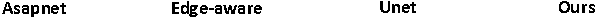
\includegraphics[width=.82\linewidth]{Chapters/detail-retouching-figs/One-shot-labels.pdf}

  \includegraphics[width=\linewidth]{Chapters/detail-retouching-figs/Qualitative_zoomed_BF.pdf}
    \caption{Qualitative comparison with baseline approaches on bilateral filtering. Bilateral filter is a nonlinear filter designed for smoothing the surfaces while preserving the edges. Results show that our proposed technique captures the bilateral-filtering effect more effectively, reducing the roughness of the surfaces while maintaining important details.} 

   \label{fig:QualitativeComp_BF}%
\end{figure*}

    
 %   These results are included in Table 1 for the filter types indicated in rows. The training strategy for the state-of-the-art methods is summarised in Section \ref{sec:Comparisons}. Before-after pairs along with additional results can be found in the supplementary material. Image courtesy of Arnaud Rougetet (landscape) and virtualhorizonstudio (alarm clock). (CC-BY and PixelSquid).

\begin{figure*}%[th]%[tph]{
  \centering
      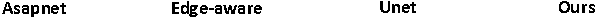
\includegraphics[width=.82\linewidth]{Chapters/detail-retouching-figs/One-shot-labels.pdf}
  \includegraphics[width=\linewidth]{Chapters/detail-retouching-figs/Qualitative_zoomed_LLF_a2_s02.pdf}
    \caption{Qualitative comparison with baseline approaches on Local Laplacian filter (LLF) ($\alpha=2, \sigma=0.2$). LLF is another edge-aware nonlinear filter designed for multiple tasks, namely edge-preserving smoothing, detail enhancement, tone mapping, and inverse tone mapping. In these examples, the parameters are chosen to have an edge-preserving smoothing effect, similar to bilateral filtering. Results show that ours offer smoother textures.} 

   \label{fig:QualitativeComp_LLF_a2}%
\end{figure*}

%These results are included in Table 1 for the filter types indicated in rows. The training strategy for the state-of-the-art methods is summarised in Section \ref{sec:Comparisons}. Before-after pairs along with additional results can be found in the supplementary material. Image courtesy of Arnaud Rougetet (landscape) and virtualhorizonstudio (alarm clock). (CC-BY and PixelSquid).

\begin{figure*}%[th]%[tph]{
  \centering
    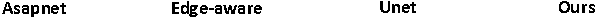
\includegraphics[width=.82\linewidth]{Chapters/detail-retouching-figs/One-shot-labels.pdf}
  \includegraphics[width=\linewidth]{Chapters/detail-retouching-figs/Qualitative_zoomed_LLF_a05_s01.pdf}
    \caption{Qualitative comparison with baseline approaches on Local Laplacian filter (LLF) ($\alpha=0.5, \sigma=0.1$). Here, the parameters are chosen accordingly to enhance the details. Our results highlight edges, such as the transition between the cloud and the sky, the numbers in the clock or the texture on the bed sheet.} 

   \label{fig:QualitativeComp_LLF_a05}%
\end{figure*}

\newpage
\subsection{Limitations and Future Work}
\begin{figure}[th] % "[t!]" placement specifier just for this example
	\centering
	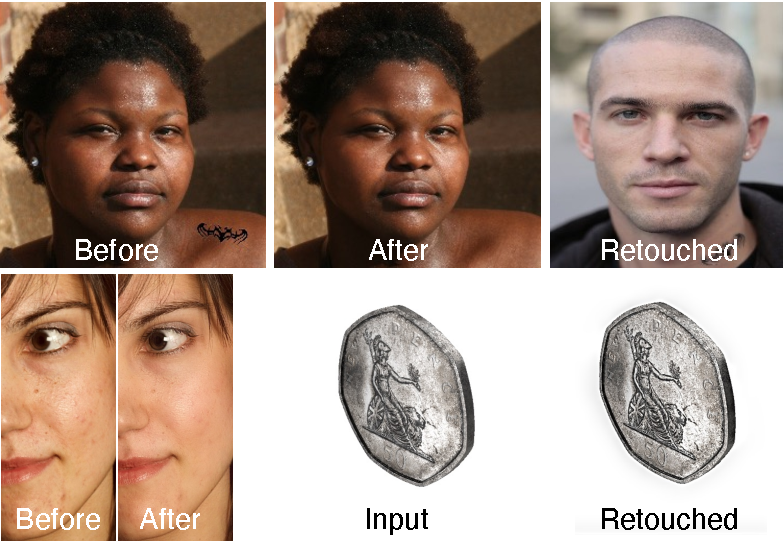
\includegraphics[width=0.8\columnwidth]{Chapters/detail-retouching-figs/Limitations.pdf}
    \caption{\label{fig:limitations} The proposed technique cannot accurately handle extreme non-repeating local effects such as tattoos (top), and when example and input images are of very different semantics (bottom). Image courtesy of bgaj23 (coin). (PixelSquid).}

\end{figure}
A primary limitation of this work is its dependence on local patches at different scales, disregarding their spatial location. Hence, the method is most useful when details are retouched based on local and repeated characteristics of an image. Non-repeating spatially-dependent strong effects, e.g., tattoos or portrait stylisations with spatially varying lighting~\cite{Shih14Style}, cannot be handled by the current technique (see Figure \ref{fig:limitations}).


Since the method relies on a single example image pair, transferring filters applied to arbitrary images~\cite{Yan14Automatic} is out of the scope of this work. Example and input images are required to have similar semantics for predictable transfer. Extending the technique to more than one pair of example images will require us to have consistently retouched details on all those example images. Finally, the example before and after images are required to be perfectly aligned. This requirement can be alleviated by incorporating an ICP~\cite{Besl92AMethod}-like approach into the optimisation in Section~\ref{sec:Methodology}. 

Although the main focus in this paper is learning artist-driven subjective retouching edits, the proposed technique is general. It can be extended to transfer arbitrary image transformations, significantly where details are modified. Thus, I plan to investigate the technique further as a general transfer method for image-to-image translation. The patch-adaptive nature of the mappings makes them amenable to analysis.



\section{Conclusions}
We presented a neural field based technique for example-based automatic retouching of images. By formulating the transfer problem in the patch space, we showed that blending multiple transformation matrices with patch-adaptive weights can be utilized to learn an accurate and generalizable map. This allowed us to use images of different scenes, people, views, and environmental conditions as the example pair and input. We illustrated the technique's utility on various retouching examples. We believe that our image map representation can be helpful in many other image processing tasks.

% \begin{figure*}%[th]
%   \centering
%   \includegraphics[height=0.8\textheight, width=\linewidth,keepaspectratio]{Images/AdditionalResults_op2.pdf}
%   \caption{
%            Retouches reproduced by our algorithm based on single before-after pairs. }
%            \label{fig:AdditionalRes}%
% \end{figure*}

% \section{Appendices}
